\documentclass[a4paper]{article}
\usepackage[utf8]{inputenc}
\usepackage{titling}
\usepackage{minted}
\usepackage{fancyvrb}
\usepackage{graphicx}
\usepackage{float}
\usepackage[binary-units=true]{siunitx}

\graphicspath{ {images/} }

\newcommand{\subtitle}[1]{
  \posttitle{
    \par\end{center}
    \begin{center}\large#1\end{center}
    \vskip0.5em}
}
 

\title{dir\_sync}
\subtitle{Protobuf-powered file synchronization}
\author{Philip Trauner}
\date{ }

\begin{document}
 
\begin{titlepage}
\maketitle
\end{titlepage}

\tableofcontents
\thispagestyle{empty}
\newpage

\section{License}
\begin{verbatim}
Boost Software License - Version 1.0 - August 17th, 2003

Permission is hereby granted, free of charge, to any person or organization
obtaining a copy of the software and accompanying documentation covered by
this license (the "Software") to use, reproduce, display, distribute,
execute, and transmit the Software, and to prepare derivative works of the
Software, and to permit third-parties to whom the Software is furnished to
do so, all subject to the following:

The copyright notices in the Software and this entire statement, including
the above license grant, this restriction and the following disclaimer,
must be included in all copies of the Software, in whole or in part, and
all derivative works of the Software, unless such copies or derivative
works are solely in the form of machine-executable object code generated by
a source language processor.

THE SOFTWARE IS PROVIDED "AS IS", WITHOUT WARRANTY OF ANY KIND, EXPRESS OR
IMPLIED, INCLUDING BUT NOT LIMITED TO THE WARRANTIES OF MERCHANTABILITY,
FITNESS FOR A PARTICULAR PURPOSE, TITLE AND NON-INFRINGEMENT. IN NO EVENT
SHALL THE COPYRIGHT HOLDERS OR ANYONE DISTRIBUTING THE SOFTWARE BE LIABLE
FOR ANY DAMAGES OR OTHER LIABILITY, WHETHER IN CONTRACT, TORT OR OTHERWISE,
ARISING FROM, OUT OF OR IN CONNECTION WITH THE SOFTWARE OR THE USE OR OTHER
DEALINGS IN THE SOFTWARE.
\end{verbatim}

\newpage

\section{Task}
Implementation of a networked command-line file synchronization utility. Timestamps and hashes should be utilized for comparison operations.

\subsection{Technologies}
\texttt{dir\_sync} is using features introduced in the C++14 standard and therefor relies on a C++ compiler adhering to this specification. \texttt{g++} (version 6.3.0-18) is used to compile \texttt{dir\_sync} on Debian 9.3 "Stretch" and \texttt{clang} (version 900.0.39.2) is used on macOS 10.13.2.

\begin{table}[h]
\centering
\begin{tabular}{l|l}
Use-Case                      & Technology \\ \hline
Networking                    & asio       \\
Logging                       & spdlog     \\
String formatting             & format     \\
Command line argument parsing & clipp      \\
Configuration files           & json       \\
SHA-512 file hashing          & OpenSSL    \\
Data exchange format          & Protobuf  
\end{tabular}
\caption{Used libraries/technologies.}
\end{table}

All libraries beside OpenSSL were mandatory as by project definition. 
OpenSSL was chosen for file hashing because no header-only library that supports SHA-512, which was deemed a requirement because SHA-256 is not considered secure anymore, could be located. It is also often pre-installed on common Linux distributions. 

\subsection{Assumptions}
\begin{enumerate}
\item Only Unix-like operating system are supported 
\item The underlying file-system of client and server is the same $\rightarrow$
\begin{enumerate}
	\item Maximum path lengths are equal
	\item Case sensitive / insensitive paths can not be mixed
\end{enumerate}
\item No control files exist in regular directories
\item Both peers have working clocks that are approximately synchronized
\item Synchronization is not continuous $\rightarrow$
\begin{enumerate}
	\item Deletion of files is not handled
\end{enumerate}
\item Conflicts are solved server-side
\item Forced synchronisation termination can result in inconsistent state
\end{enumerate}


\section{Implementation}
\subsection{Code sharing}
Functions and constants used by server as well as client are defined in a module aptly named \texttt{shared} to prevent needless code duplication. 

\subsection{Recursive directory traversal}
The \texttt{filesystem} library was introduced into the C++ language standard in 2016. Support is still relatively poor, neither the LLVM toolchain bundled with macOS nor the GNU toolchain bundled with Debian 9.3 include a current non-experimental version of the library. 
It was decided to sacrifice support of non Unix-like operating systems and use the \texttt{nftw(...)} (\texttt{<ftw.h>}) function instead. It expects a pointer to a function that is called for every item in the file tree it traverses, therefor persistent data has to stored in an overlying scope, which, in this case, is the root scope. To prevent possible data races the \texttt{nftw()} call itself is wrapped in another function that locks a global \texttt{Mutex} on execution.

\subsection{Protocol Buffers}
\begin{figure}[H]
\centering
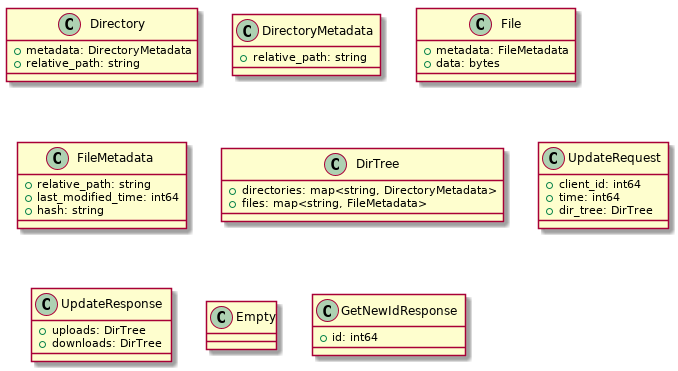
\includegraphics[height=8cm]{protobufs}
\caption{All defined Protobuf messages.}
\end{figure}

Communication between server and client is exclusively handled with Protobuf messages. 
An example of their usage in the actual protocol can be found on page~\pageref{sec:phases}.
\newpage

\subsection{Command line interface}
\begin{verbatim}
SYNOPSIS
        ./dir_sync_server <directory> [--strict] 
        			    [--verbose] [-p <port>] [-c <config>]
        ./dir_sync_client <directory> <address>  
        			    [--verbose] [-p <port>] [-c <config>]

OPTIONS
        --strict    do not continue if client is deemed insane
        --verbose   log additional debug info
        -p, --port  provide alternative port

        -c, --config
                    override command line parameters with config
\end{verbatim}

\texttt{dir\_sync\_server} and \texttt{dir\_sync\_client} provide very similar command line interfaces. The address is not configurable for \texttt{dir\_sync\_server} because its IPv4 socket is automatically bound to 0.0.0.0. 
\bigbreak
A configuration file in the \texttt{JSON} file format can also be supplied to substitute optional parameters. All command line options are available as keys.

\begin{figure}[H]
\begin{minted}[]{json}
{
	"strict": true,
	"verbose": true,
	"port": 1337,
}

\end{minted}
\caption{Example configuration file.}
\end{figure}

\section{Networking}
A slim header is perpended to Protobuf messages to determine their length and differentiate between different message types. 

Fixed size unsigned integers are used because their length should be identical between different operating systems and processor architectures. 

asio's \texttt{mutable\_buffer}s are used to encode all header fields before transmission.
\begin{figure}[H]
\centering
\begin{BVerbatim}
+---+------------------------+
| 1 |            8           |
+---+------------------------+
\end{BVerbatim}
\caption{Header perpended to Protobuf messages.}
\end{figure}

To cut down on boilerplate code it was decided to utilize lookup tables to dynamically determine which type of Protobuf message is being sent or received. 

\begin{figure}[H]
\begin{minted}[]{c++}
enum class MessageType {
	FileTree = 1,
	FileRequest = 2,
	// ...
};

const unordered_map<type_index, MessageType> proto_type_mapping {
	{typeid(FileTree), MessageType::FileTree},
	{typeid(FileRequest), MessageType::FileRequest},
	// ...
};
\end{minted}
\caption{Shortened lookup table definition.}
\end{figure}

This decision rules out possible optimizations by the compiler, as message type lookup has to be performed at runtime. While this compromise does result in degraded performance, the difference is insignificant as most processor time will be spent waiting for file I/O operations to complete.

\begin{figure}[H]
\begin{minted}[]{c++}
void send_proto(tcp::socket& sock, Message& message) {
	u_int8_t message_type{to_underlying(
		proto_type_mapping.at(typeid(message)))};
	u_int64_t message_size{message.ByteSizeLong()};

	write(sock, buffer(&message_type, U_INT_8_SIZE));
	write(sock, buffer(&message_size, U_INT_64_SIZE));

	streambuf buf;
	ostream os(&buf);
	message.SerializeToOstream(&os);

	write(sock, buf);
}
\end{minted}
\caption{Send function (error handling stripped out to reduce length). All Protobuf messages are subclasses of Message.}
\end{figure}

This design decision implies that the receiving end always knows which message type will be received next, which is not possible in scenarios where the same message type is sent multiple times in a row (\texttt{FileBlock}, \texttt{FileRequest}, ...). A special message type called \texttt{ProtocolSeparator} was introduced to solve this issue. It has no content and is sent to delimit protocol stages.
\bigbreak
An example of its usage in the actual protocol can be found on page~\pageref{fig:stage2}.
\bigbreak
The \texttt{recv\_proto} function returns a special status code if a \texttt{ProtocolSeparator} has been received instead of the expected message type. It is the responsibility of the application logic to validate the returned status code for each received message.

\subsection{Protocol phases}
\label{sec:phases}
\subsubsection{First phase}
\begin{figure}[H]
\centering
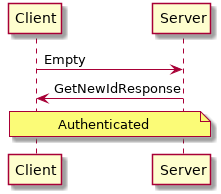
\includegraphics[width=4.5cm]{first_stage}
\caption{First phase: Transmission of \texttt{SanityCheck} and \texttt{FileTree}.}
\end{figure}

After the client establishes a connection to the server it creates a \texttt{SanityCheck} message and fills it with its current time which is then forwarded to the server. The client is deemed sane if its clock offset relative to the server time is less than five seconds. If the client is deemed insane a warning message is displayed by the server.

The client then traverses all files and directories in the specified folder to compose a \texttt{FileTree} message, which is used by the server to compute which files/directories need the be created/sent/requested.

\subsubsection{Second phase}
\begin{figure}[H]
\centering
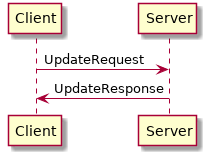
\includegraphics[width=4.5cm]{second_stage}
\caption{Second phase: Transmission of directories and files as well as requests for files that are not present on the server.}
\label{fig:stage2}
\end{figure}

After the server has created all folders that are present in the received \texttt{FileTree} but are missing locally it emits \texttt{DirectoryMetadata} messages filled with directories that have to be created by the client. After all necessary \texttt{DirectoryMetadata} messages have been transmitted a \texttt{ProtocolSeparator} is sent.

\begin{figure}[H]
\begin{minted}[]{c++}
for (const string& dir_path : get<0>(file_tree_dir_diff_)) {
	send_directory(sock, dir_path);
}

send_protocol_separator(sock);
\end{minted}
\caption{Transmission of \texttt{DirectoryMetadata} messages.}
\end{figure}

Files that are present on the server but missing on the client are handled next. A \texttt{MinimalFileMetadata} message containing the path of the file that is about to be transfered as well as its last modification time-stamp is sent before \SI{65536}{\byte} file parts are transmitted in the form of \texttt{FileResponse} messages. A \texttt{ProtocolSeparator} marks the end of a file. If two consecutive \texttt{ProtocolSeparator}s are received the client assumes that all missing files have been received.

Lastly, the server requests all missing files from the client. 


\subsubsection{Third phase}
\begin{figure}[H]
\centering
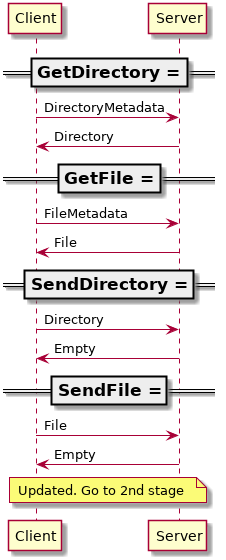
\includegraphics[width=4.5cm]{third_stage}
\caption{Third phase: Files that have been requested by the server are sent by the client.}
\end{figure}

After all \texttt{FileRequest} messages have been received the client sends the requested files in the same manner as the server does in phase two.

\section{Conclusion}
Just use \texttt{rsync -avP --checksum <source> <destination>}.

\end{document}